%%%%%%%%%%%%%%%%%%%%%%%%%%%%%%%%%%%%%%%%%%%%%%%%%%%%%%%%%%%%%%%%%
% MUW Presentation
% LaTeX Template
% Version 1.0 (27/12/2016)
%
% License:
% CC BY-NC-SA 4.0 (http://creativecommons.org/licenses/by-nc-sa/3.0/)
%
% Created by:
% Nicolas Ballarini, CeMSIIS, Medical University of Vienna
% nicoballarini@gmail.com
% http://statistics.msi.meduniwien.ac.at/
%
% Customized for UAH by:
% David F. Barrero, Departamento de Automática, UAH
%%%%%%%%%%%%%%%%%%%%%%%%%%%%%%%%%%%%%%%%%%%%%%%%%%%%%%%%%%%%%%%%%

\documentclass[10pt,compress]{beamer} % Change 10pt to make fonts of a different size
\mode<presentation>

\usepackage[spanish]{babel}
\usepackage{fontspec}
\usepackage{tikz}
\usepackage{etoolbox}
\usepackage{xcolor}
\usepackage{xstring}
\usepackage{listings}

% Custom packages
\usepackage{tikz}
\def\layersep{2.5cm}
\usetikzlibrary{matrix,chains,positioning,decorations.pathreplacing,arrows}

\usetheme{UAH}
\usecolortheme{UAH}
\setbeamertemplate{navigation symbols}{} 
\setbeamertemplate{caption}[numbered]

%%%%%%%%%%%%%%%%%%%%%%%%%%%%%%%%%%%%%%%%%%%%%%%%%%%%%%%%%%%%%%%%%
%% Presentation Info
\title[Introduction to Evolutionary Computation]{Introduction to Evolutionary Computation}
\author{\asignatura\\\carrera}
\institute{}
\date{Departamento de Automática}
%%%%%%%%%%%%%%%%%%%%%%%%%%%%%%%%%%%%%%%%%%%%%%%%%%%%%%%%%%%%%%%%%

%%%%%%%%%%%%%%%%%%%%%%%%%%%%%%%%%%%%%%%%%%%%%%%%%%%%%%%%%%%%%%%%%
%% Descomentar para habilitar barra de navegación superior
\setNavigation
%%%%%%%%%%%%%%%%%%%%%%%%%%%%%%%%%%%%%%%%%%%%%%%%%%%%%%%%%%%%%%%%%

%%%%%%%%%%%%%%%%%%%%%%%%%%%%%%%%%%%%%%%%%%%%%%%%%%%%%%%%%%%%%%%%%
%% Configuración de logotipos en portada
%% Opacidad de los logotipos
\newcommand{\opacidad}{1}
%% Descomentar para habilitar logotipo en pié de página de portada
\renewcommand{\logoUno}{Images/isg.png}
%% Descomentar para habilitar logotipo en pié de página de portada
%\renewcommand{\logoDos}{Images/CCLogo.png}
%% Descomentar para habilitar logotipo en pié de página de portada
%\renewcommand{\logoTres}{Images/ALogo.png}
%% Descomentar para habilitar logotipo en pié de página de portada
%\renewcommand{\logoCuatro}{Images/ELogo.png}
%%%%%%%%%%%%%%%%%%%%%%%%%%%%%%%%%%%%%%%%%%%%%%%%%%%%%%%%%%%%%%%%%


%%%%%%%%%%%%%%%%%%%%%%%%%%%%%%%%%%%%%%%%%%%%%%%%%%%%%%%%%%%%%%%%%
%% FOOTLINE
%% Comment/Uncomment the following blocks to modify the footline
%% content in the body slides. 


%% Option A: Title and institute
\footlineA
%% Option B: Author and institute
%\footlineB
%% Option C: Title, Author and institute
%\footlineC
%%%%%%%%%%%%%%%%%%%%%%%%%%%%%%%%%%%%%%%%%%%%%%%%%%%%%%%%%%%%%%%%%

\begin{document}

%%%%%%%%%%%%%%%%%%%%%%%%%%%%%%%%%%%%%%%%%%%%%%%%%%%%%%%%%%%%%%%%%
% Use this block for a blue title slide with modified footline
{\titlepageBlue
    \begin{frame}
        \titlepage
    \end{frame}
}

\institute{\asignatura}

\begin{frame}[plain]{}
   \begin{block}{Objectives}
       \begin{itemize}
        \item Introduce biological evolution
        \item Introduce artificial evolution
		\item Justify the utility of artificial evolution from an engineering perspective
		\item Overview the components of an Evolutionary Algorithm
       \end{itemize}
   \end{block}

   \begin{block}{Bibliography}
   		\begin{itemize}
       \item Eiben, A.E. and Smith, J.E. \emph{Introduction to Evolutionary Computing}. Springer 2003. 
     	\item Luke, S. \emph{Essentials of Metaheuristics}. 2nd edition. Ed. Lulu, 2010. \href{https://cs.gmu.edu/~sean/book/metaheuristics/Essentials.pdf}{(Link)}
   		\end{itemize}
   \end{block}
\end{frame}

{
\disableNavigation{white}
\begin{frame}[shrink]{Table of Contents}
 \frametitle{Table of Contents}
 \tableofcontents
  % You might wish to add the option [pausesections]
\end{frame}
}

\section{Biological background}
\subsection{Historical review}
\begin{frame}{Biological background}{Historical review (I)}
 	\begin{columns}
 	   \column{.60\textwidth}
		Anaximander of Miletus (610 – 546 BC)

 	 	\begin{itemize}
		\item First animals come from water
		\item Man come from fishes
		\end{itemize}

		Plato (428/427 – 348/347 BC)
		\begin{itemize}
		\item Demiurgo created the cosmos
		\item Theory of Ideas
		\end{itemize}
		
		Aristotle (384 – 322 BC)
		\begin{itemize}
		\item Spontaneous generation
		\item Strong influence in Europe
		\end{itemize}
 	   \column{.30\textwidth}
		\centering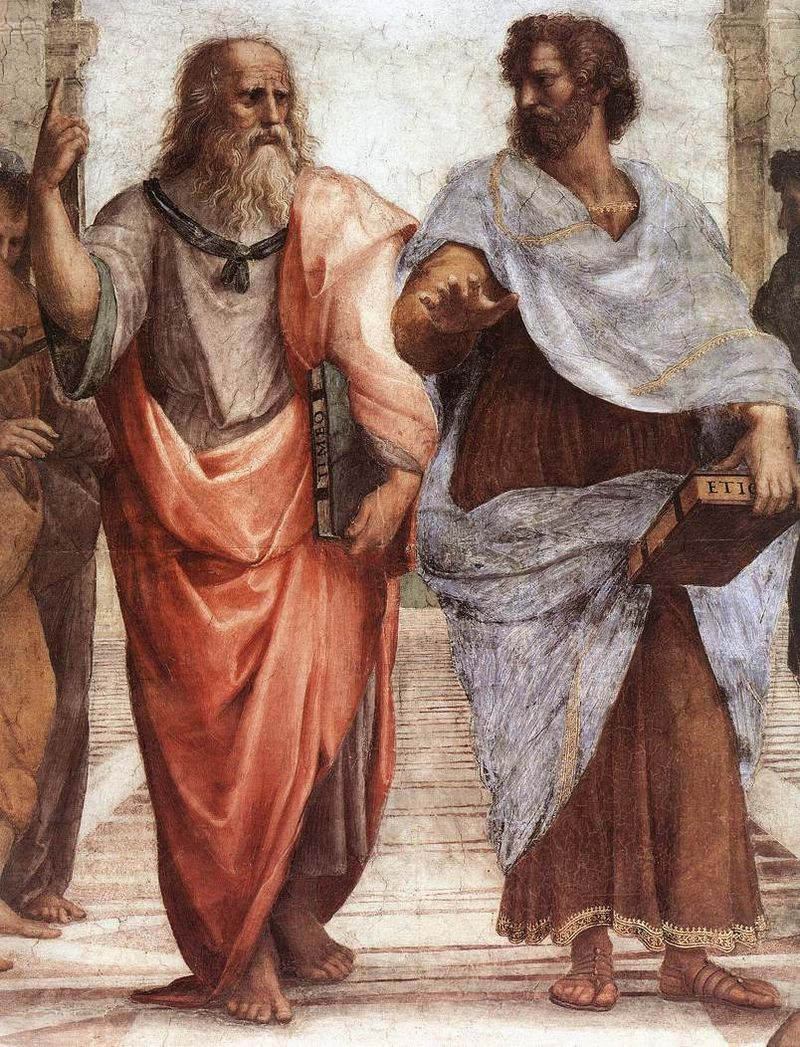
\includegraphics[width=\linewidth]{figs/plato.jpg}
	\end{columns}
\end{frame}

\begin{frame}{Biological background}{Historical review (II)}
	\vspace{-0.2cm}
	\begin{center}\includegraphics[width=0.4\linewidth]{figs/adam.jpg}\\
	\end{center}
	   Creationism: God created all the species
 	 	\begin{itemize}
		\item Literal interpretaton of the Genesis
		\item Species are hierarchical
		\item Man has a superior position
		\end{itemize}
		Main school in Europe for centuries
\end{frame}

\begin{frame}{Biological background}{Historical review (III)}
 	\begin{columns}
 	   \column{.65\textwidth}
		Georges Louis Leclerc (1707 - 1788)

 	 	\begin{itemize}
		\item Especulated that species change
		\item Noticied the similarities between men and apes
		\item Could not provide a theory
		\end{itemize}

		Jean-Baptiste Lamarck (1744 - 1829)
		\begin{itemize}
		\item First to propose a theory of evolution
		\item Transmutation of Species
		\item Use strengthens/weakens organs
		\item Heritability of acquired characteristics
		\end{itemize}

 	   \column{.25\textwidth}
		\centering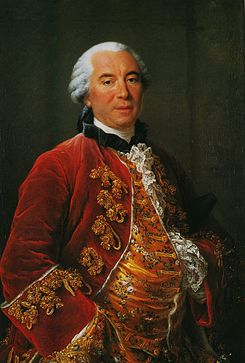
\includegraphics[width=\linewidth]{figs/leclerc.jpg}\\
		\centering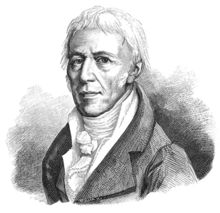
\includegraphics[width=\linewidth]{figs/lamarck.jpg}
	\end{columns}
\end{frame}

\begin{frame}{Biological background}{Historical review (IV)}
	Charles Darwin (1809-1882)
	\begin{itemize}
		\item Published in \textit{``On the Origin of the Species''} in 1859
			\begin{itemize}
			\item[] \small{(\textit{''On the Origin of Species by Means of Natural Selection, or the Preservation of Favoured Races in the Struggle for Life''})}
			\end{itemize}
		\item Introduced \alert{natural selection} ... and applies it to human being
			\begin{itemize}
			\item Natural selection = Variability + selection
			\end{itemize}
		\item Darwin did not explain the source of variation
	\end{itemize}
	\begin{center}
	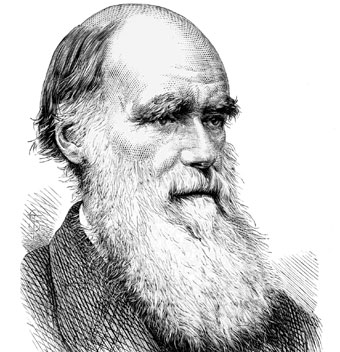
\includegraphics[width=0.2\linewidth]{figs/darwin.jpg}\hspace{1cm}
	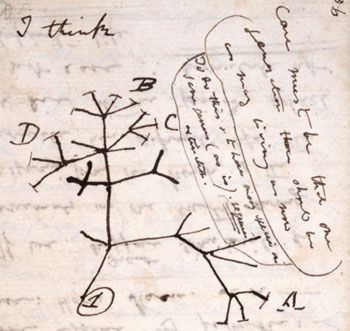
\includegraphics[width=0.2\linewidth]{figs/ithink.jpg}
	\end{center}
\end{frame}

\begin{frame}{Biological background}{Historical review (V)}
 	\begin{columns}
 	   \column{.7\textwidth}
		Gregor Mendel (1822 - 1884)
		\begin{itemize}
		\item Mendelian inheritance
		\item Recessive and dominant traits
		\end{itemize}


		August Weismann (1834 - 1914)
 	 	\begin{itemize}
		\item Germ plasm theory
		\item Germ and somatic cells
		\item End of Lamarkism
		\end{itemize}
		
		J. Watson (1928) and F. Crick (1916 - 2004)
 	 	\begin{itemize}
		\item Discovery of DNA
		\item Central Dogma of molecular biology
		\end{itemize}


 	   \column{.3\textwidth}
		\centering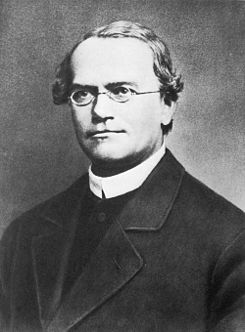
\includegraphics[width=0.5\linewidth]{figs/mendel.jpg}
		\centering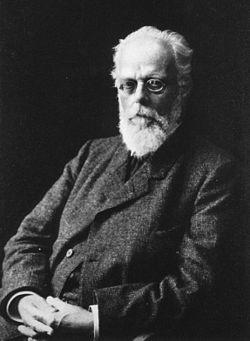
\includegraphics[width=0.5\linewidth]{figs/weismann.jpg}\\
		\centering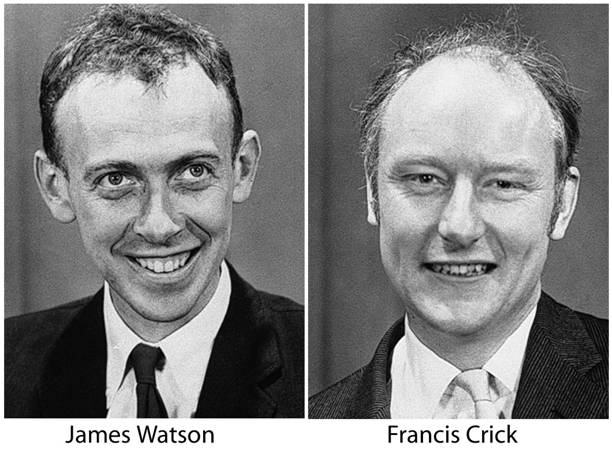
\includegraphics[width=\linewidth]{figs/WatsonCrick.jpg}
	\end{columns}
\end{frame}



\subsection{Theory of Evolution}
\begin{frame}{Biological background}{Theory of Evolution}
	Neo-Darwinism: Darwin + Mendel + Weismann
	\begin{itemize}
		\item ... also called Theory of Evolution
		\item Variability + selection = \alert{evolution}
	\end{itemize}
	There is variation among individuals
	\begin{itemize}
		\item Sexual reproduction, mutation and gene flow
  	\end{itemize}
	There is a selection of those individuals
	\begin{itemize}
		\item \alert{Natural selection}
		\item Artificial selection
		\item Sexual selection
		\item Genetic drift (deriva genética) \href{http://evolution.berkeley.edu/evolibrary/images/evo/beetles\_mech3.gif}{(Link)}
	\end{itemize}
	The \textit{fittest} is the one that survives (not the strongest!)
\end{frame}

\subsection{Molecular Genetics}
\begin{frame}{Biological background}{Molecular Genetics (I)}
    \begin{columns}
 	   \column{.70\textwidth}
		Organisms are made by \textbf{proteins}

 	 	\begin{itemize}
		\item Proteins are sequences of \textbf{aminoacids}
		\item They folder in a 3D structure
		\item $20$ aminoacids
		\end{itemize}
		DNA codifies all the proteins in an organism\\
 	   \column{.40\textwidth}
		\centering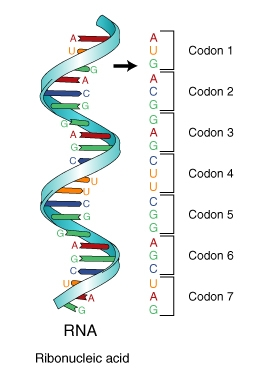
\includegraphics[width=\linewidth]{figs/codones.jpg}
	\end{columns}
\end{frame}

\begin{frame}[plain]{Biological background}{Molecular Genetics (II)}
		\textbf{Protein synthesis}: Creation of proteins from DNA \href{https://www.youtube.com/watch?v=gG7uCskUOrA}{(video)}
		\begin{center}
		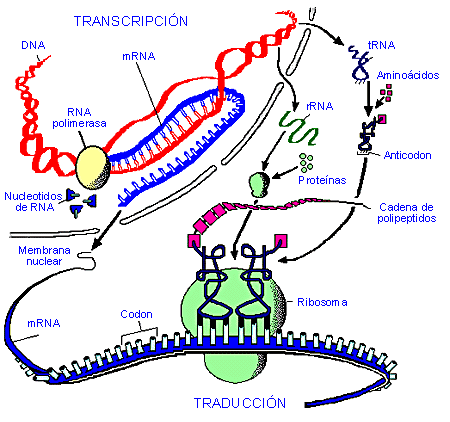
\includegraphics[width=0.7\linewidth]{figs/sintesis.png}\\
		\tiny \href{http://www.virtual.unal.edu.co/cursos/ingenieria/2001832/lecciones/traduccion.html}{(Source)}
		\end{center}
\end{frame}

\begin{frame}{Biological background}{Molecular Genetics (III)}
	Useful biological terms
	\begin{description}
	\item[Gene] ADN fragment that codifies one protein
	\item[Allele] The variant form of a gene
	\item[Genotype] The sequence of DNA
	\item[Phenotype] Characteristics of an individual
	\item[Exon] Part of a gene that is transcripted
	\item[Intron] Part of a gene that is not trascripted
	\end{description}

	\begin{center}
	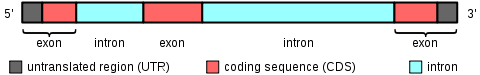
\includegraphics[width=0.7\linewidth]{figs/exon.png}\\
	\tiny \href{https://en.wikipedia.org/wiki/Exon}{(Source)}
	\end{center}
\end{frame}

\subsection{{Theory of Evolution from an algorithmic perspective}}
\begin{frame}{Biological background}{Theory of Evolution from an algorithmic perspective}
	Given a population ...
	\begin{enumerate}
	\item There are differences among individuals
	\item Fittest individuals more likely to reproduce
	\item Go to 1
	\end{enumerate}
	We are interested in applying this to Engineering
\end{frame}

\begin{frame}[plain]{}
	\note{Poner como ejemplo el perfil de un ala, geometria de una antena microscript e insercion orbital}
	\vspace{2cm}
	\begin{center}
	How can we apply biological evolution to solve engineering problems?
	\end{center}
\end{frame}

\section{Evolutionary Algorithms}
\subsection{Evolution as optimization}
\begin{frame}{Evolutionary Algorithms}{Evolution as optimization}
    \begin{columns}
 	   \column{.50\textwidth}
	\begin{center}
	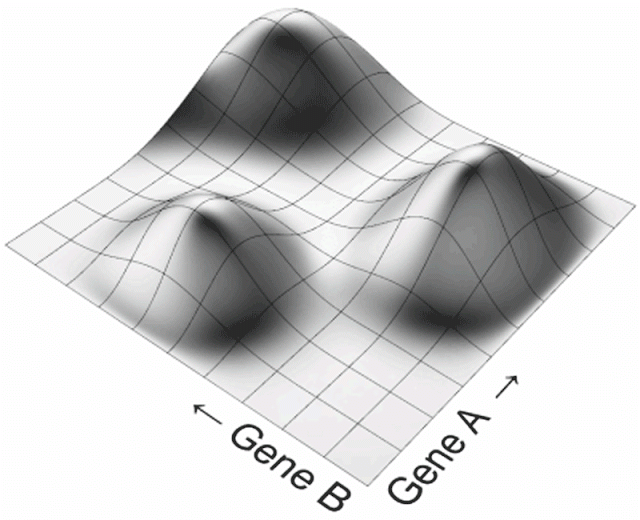
\includegraphics[width=\linewidth]{figs/fitness-landscape-0.png}\\
		\tiny \href{http://2.bp.blogspot.com/-32R9V6X6rXU/T-tr1lZIwCI/AAAAAAAAAFI/t05ioQ5GP80/s1600/Fitness-Landscape.gif}{(Source)}
	\end{center}
 	   \column{.50\textwidth}
	Biological evolution is, in essence, an optimization algorithm
	\begin{itemize}
	\item ... it optimizes the survival probability
	\item Optimizing is to \textit{search} the maximum
	\end{itemize}
	\end{columns}
\end{frame}

\subsection{AI, search and optimization}
\begin{frame}{Evolutionary Algorithms}{AI, search and optimization (I)}
    \begin{columns}
 	   \column{.50\textwidth}
	AI is much related to search a solution for a problem
	\begin{itemize}
	\item Search space
	\item Solution space
	\end{itemize}
	Almost any computational problem can be expressed as a search problem
	 	   \column{.50\textwidth}
	\begin{center}
	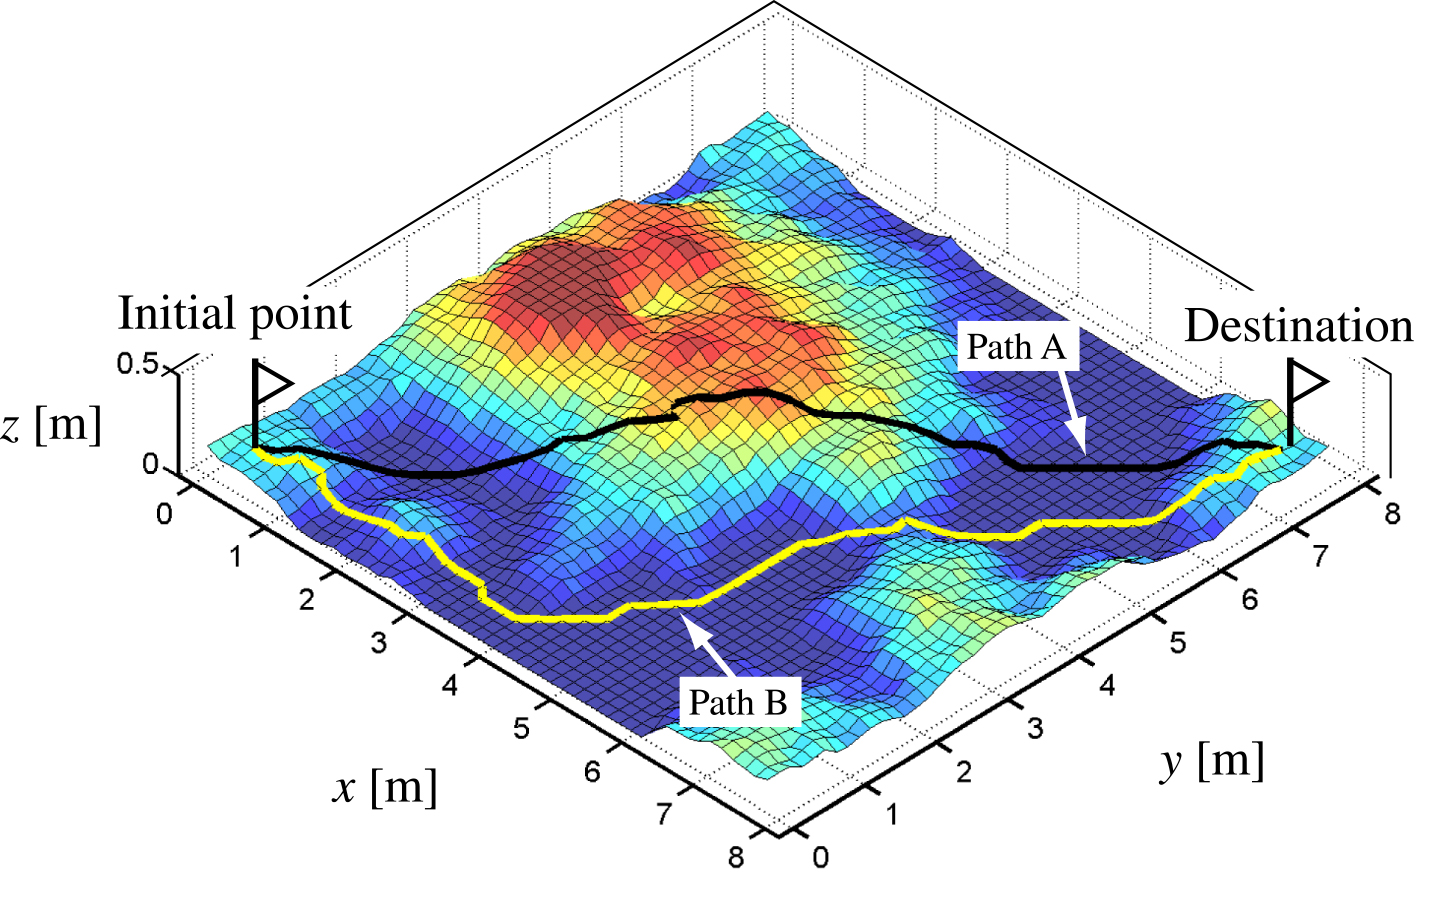
\includegraphics[width=\linewidth]{figs/path.jpg}\\
	\tiny{\href{http://www.astro.mech.tohoku.ac.jp/~ishigami/research/path\_plan.html}{(Source)}}
	\end{center}
	   \end{columns}
\end{frame}

\begin{frame}{Evolutionary Algorithms}{AI, search and optimization (II)}
    \begin{columns}
 	   \column{.60\textwidth}
	In AI, potential solutions are assessed
	\begin{itemize}
		\item Cost function
		\item Objective: Maximize cost function
	\end{itemize}
	The solution to any problem: \textbf{exhaustive search}
	\begin{itemize}
	\item Inviable in practice
	\end{itemize}
	How to find a solution efficiently?
	\begin{itemize}
		\item With domain knowledge
		\item With randomness: \alert{Metaheuristics}
	\end{itemize}

 	   \column{.50\textwidth}
	\begin{center}
		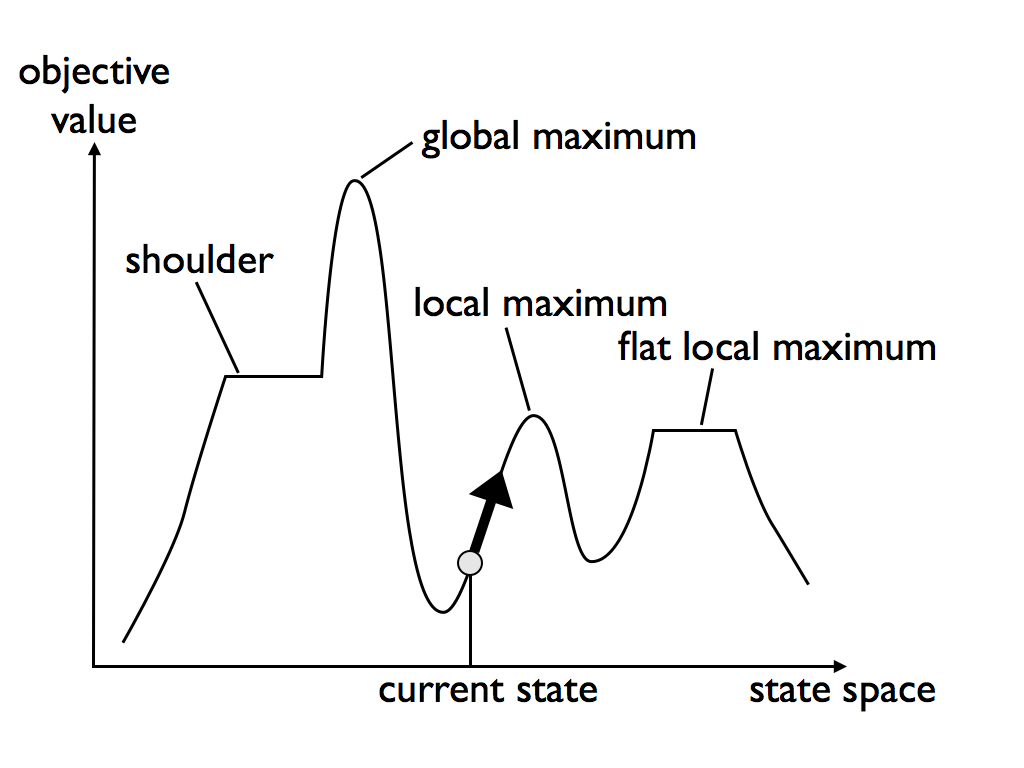
\includegraphics[width=\linewidth]{figs/landscape.png}\\
		\tiny{\href{http://www.handmade-insights.com/blog/2013/genetic-algorithmslandscape}{(Source)}}\\
	\end{center}
	\end{columns}
\end{frame}

\subsection{Metaheuristics}
\begin{frame}[plain]{Evolutionary Algorithms}{Metaheuristics}
	\begin{center}
		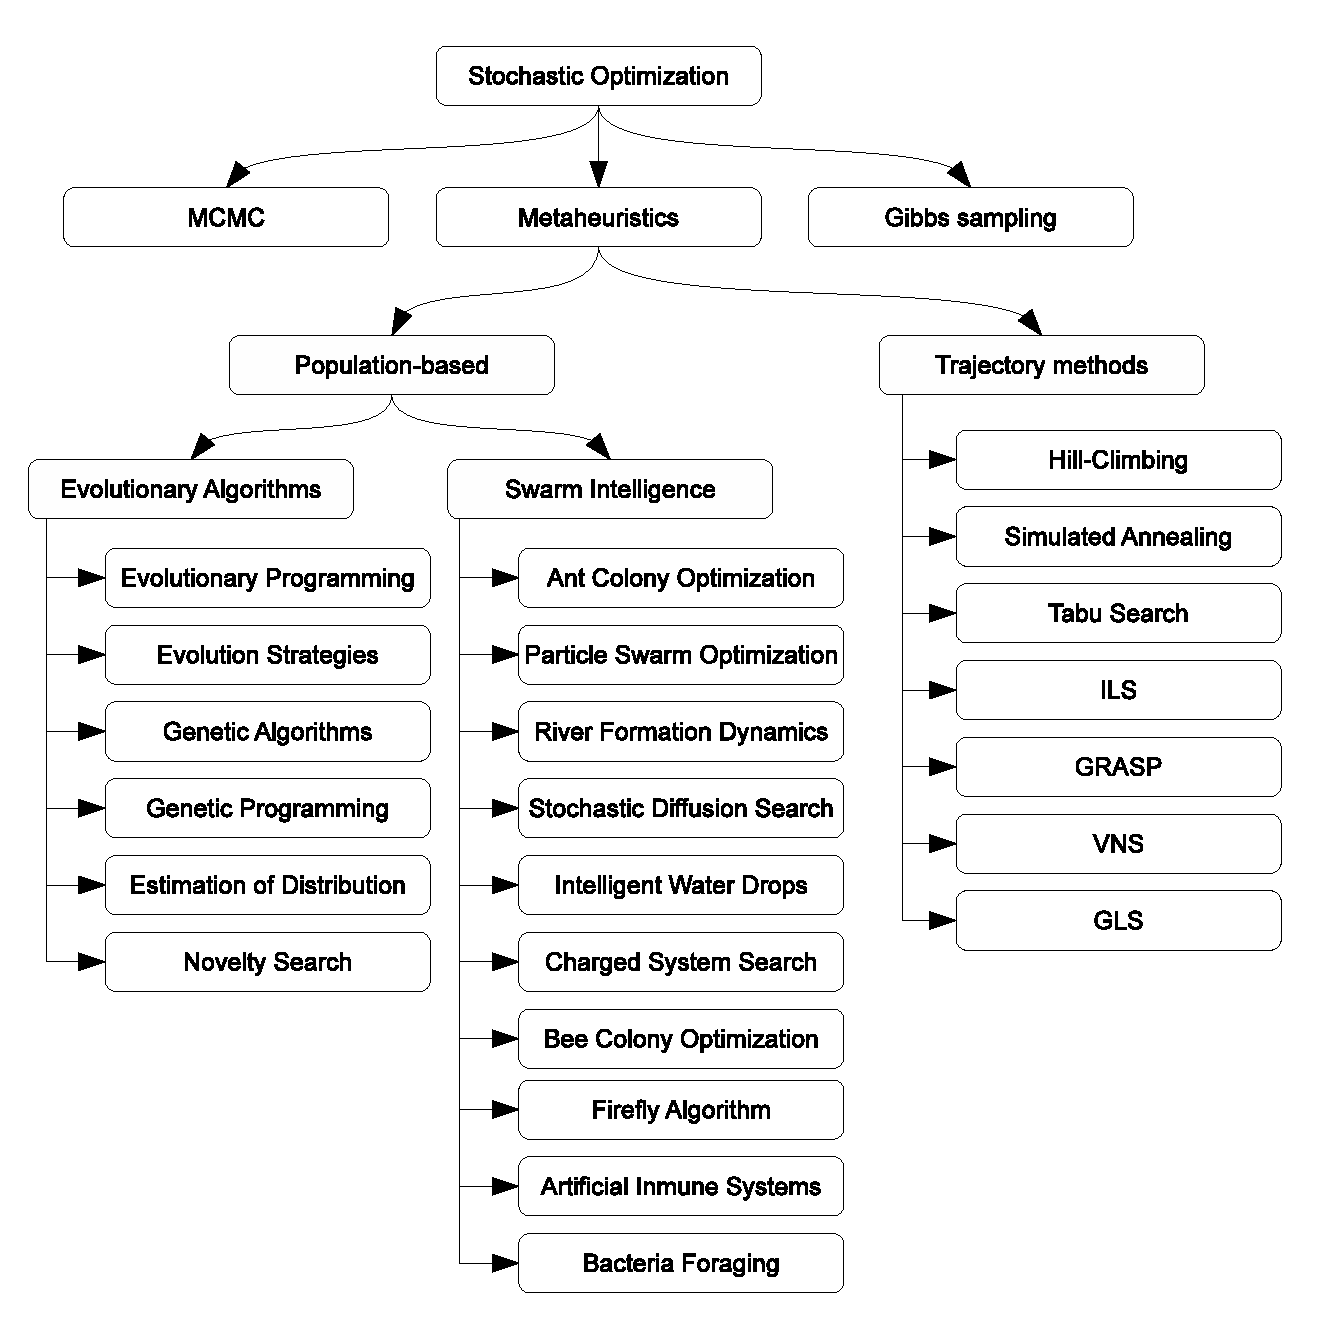
\includegraphics[width=0.75\linewidth]{figs/metaheuristics.eps}
	\end{center}
\end{frame}

\begin{frame}[plain]{}
	\vspace{2cm}
	\begin{center}
	Again:\\
	How can we apply biological evolution to solve engineering problems?
	\end{center}
\end{frame}

\subsection{Basics}
\begin{frame}{Evolutionary Algorithms}{Basics (I)} 
	Large number of Evolutionary Algorithms
	\begin{itemize}
		\item There is no ``canonical'' algorithm
		\item They all imitate biological evolution
	\end{itemize}
	They use a population
	\begin{itemize}
		\item Each individual represents a (potential) solution
		\item Multiple \textbf{representations}
	\end{itemize}
	Population is modified
	\begin{itemize}
		\item Mutation (1 individual)
		\item Crossover (>1 individuals)
		\item Multiple \textbf{genetic operators}
	\end{itemize}
	Selection that imitates natural selection
	\begin{itemize}
		\item Based on a \textbf{fitness} function
	\end{itemize}
	Iterative process
\end{frame}

\begin{frame}{Evolutionary Algorithms}{Basics (II)} 
	\begin{center}
		Possible basic algorithm
		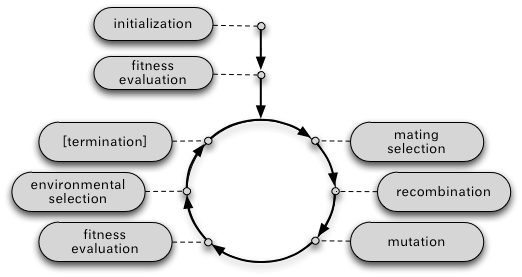
\includegraphics[width=0.75\linewidth]{figs/evolution.png}
	\end{center}
\end{frame}

\begin{frame}{Evolutionary Algorithms}{Basics (III)}
	Initialization is usually random
	\begin{itemize}
		\item Random population
		\item Domain-dependent heuristics may be used
		\item Known solutions migh be injected into the initial population
	\end{itemize}
	Termination criteria
	\begin{itemize}
		\item Get a desired fitness
		\item Maximum number of iterations (or generations)
		\item Loss of genetic diversity
		\item Lack of fitness improvment
	\end{itemize}
\end{frame}

\subsection{Exploration and explotation}
\begin{frame}{Evolutionary Algorithms}{Exploration and explotation} 
	Balance between \alert{explotation} and \alert{exploration}
        \begin{itemize}
	    \item These are oposite objectives $\Rightarrow$ Need of trade-off
        \end{itemize}
	Exploration: Search of new regions (\alert{global search})
		\begin{itemize}
		\item Explore the search space
		\item Performed, mostly, by mutation
		\end{itemize}
	Explotation: Search of local (or global) maxima (\alert{local search})
		\begin{itemize}
		\item Exploit the adquired knowledge
		\item Performed, mostly, by crossover
		\end{itemize}
\end{frame}

\IfStrEq{\modo}{MASTER-INDUSTRIALES}{
	%%%%%%%%%%%%%%%%%%%%%%%%%%%%%%%%%%%%%%%%%%%%%%%%%%%%%%%%%%%%%%%%%%%%%%%%%%%%%%%
%     enunciado.tex:    Enunciado de la pr�ctica 2 de GIEAI-Inform�tica
%%%%%%%%%%%%%%%%%%%%%%%%%%%%%%%%%%%%%%%%%%%%%%%%%%%%%%%%%%%%%%%%%%%%%%%%%%%%%%%

\documentclass[english,a4paper,11pt]{article}

\usepackage[latin1]{inputenc}  % codificaci�n de caracteres de este archivo
\usepackage[spanish]{babel}    % Traducir: ``abstract'' ---> ``resumen''   etc.
\usepackage{fancyhdr}          % p�ginas con cabecera y pie
\usepackage{listings}          % listados de c�digo fuente
\usepackage{float}             % para que los listados floten como las figuras
\usepackage{vmargin}           % ajuste de m�rgenes f�cil de usar
\usepackage[T1]{fontenc}       % meter fuentes vectoriales
\usepackage{graphicx}          % figuras
\usepackage{upquote}           % comilla recta con \textquotesingle
\usepackage{placeins}          % orden \FloatBarrier para mantener figuras a raya

\usepackage[implicit=false]{hyperref}  % enlaces web (el par�metro implicit=false
                                       % evita problemas con el # de #include etc.)
                                       % uso expl�cito: \href[options]{URL}{text}
                                       %                \url{URL}

% mis abreviaturas
\newcommand{\C}{\texttt{C}}            % escribir� \C en lugar de \texttt{C}
\newcommand{\Pascal}{\texttt{Pascal}}  % idem con \Pascal ...
\newcommand{\fun}[1]{\texttt{#1()}}    % "\fun{main}" ---> "main()" en letra typewriter
\newcommand{\hex}[1]{\texttt{#1}$_{hex}$}
\newcommand{\bin}[1]{\texttt{#1}$_{bin}$}
\newcommand{\enesimo}{\mbox{n-�simo}}
\newcommand{\muvision}{\textit{$\mu\!$Vision4}}
\newcommand{\keilmuvision}{\textit{Keil}~\muvision}
\newcommand{\codigo}[1]{\texttt{#1}}
\newcommand{\menu}[1]{\textit{#1}}

% �rdenes para alternar entre el estilo espa�ol (ligera separaci�n extra
% entre p�rrafos) y el estilo por defecto (p�rrafos junticos junticos)
\newcommand{\parrafosjuntos}{\setlength{\parskip}{0pt}}
\newcommand{\parrafosseparados}{\setlength{\parskip}{1.5ex plus 0.6ex minus 0.5ex}}

% datos importantes del documento
\newcommand{\titulo}{One-max problem with a basic Genetic Algorithm}     % <<--- T�TULO
\newcommand{\fecha}{}                         % <<--- TEMA
\newcommand{\asignatura}{IASCA}
\newcommand{\institucion}{Departamento de Autom�tica, UAH}
\newcommand{\paginaweb}{http://atc1.aut.uah.es}

% portada
\title{\asignatura \\ \titulo}
\author{\institucion \\ \url{\paginaweb}}
\date{\fecha}

% m�rgenes un poco m�s finos
\setmargrb{25mm}{20mm}{25mm}{20mm}    % left, top, right, bottom

% encabezado y pie
\pagestyle{fancy}
\lhead{\footnotesize \parbox{11cm}{\asignatura}}
\lfoot{\footnotesize \parbox{11cm}{\institucion}}
\cfoot{}
\rhead{\footnotesize \titulo}
\rfoot{\footnotesize P�gina \thepage}
\renewcommand{\headheight}{24pt}
\renewcommand{\footrulewidth}{0.4pt}
%\renewcommand{\headrulewidth}{0pt}

% listados de c�digo fuente flotantes
%\newfloat{floatlisting}{h}{}
%\floatname{floatlisting}{Listado}

% estilo de los listados de c�digo
\lstset{numbers=left,                 % n�meros de l�nea
        numberstyle=\tiny,            % tama�o de los num. de l�nea
        extendedchars=true,           % acentos, e�es...
        %frame=single,                 % marco que encuadra al listado
        basicstyle=\footnotesize\ttfamily,   % tipo de letra
        showstringspaces=false}       % no mostrar espacios de las cadenas

\graphicspath{{figs/}}                % ruta de las figuras

\begin{document} % ------------------ Aqu� empieza el documento ----------------------

% redefinir el nombre de algunas cosas
\renewcommand{\tablename}{Tabla}                  % mejor "Tabla" que "Cuadro"
\renewcommand{\listtablename}{Indice de tablas}
% definidos originalmene en:
%/usr/share/texmf-texlive/tex/generic/babel/spanish.ldf

\maketitle              % montar el t�tulo aqu�� con los par�metros definidos arriba
\thispagestyle{empty}   % no poner n�mero de p�gina ni nada de nada en la 1� p�gina

\renewcommand{\abstractname}{}         % eliminar "Resumen"
\begin{abstract}                       % resumen (sin la palabra "Resumen")
\noindent \textbf{Objectives:}
\begin{itemize}
\item Understand the structure of a basic GA
\item Accustom oneself to the way EAs address problems
\end{itemize}
\end{abstract}

\sloppy              % hacer m�s flexible el c�lculo del espacio entre palabras para
                     % evitar errores de tipo "overfull box"
                     % (lo contrario de \sloppy es \fussy)

\parrafosseparados   % separaci�n entre p�rrafos (por defecto saldr�n pegados)

\subsection*{Practice}
Often, when someone begins to learn a new programming language he implements the famous ``Hello World'' program. The equivalent to this in Evolutionary Computation is the one-max, a trivial problem often used to practice a new EC framework or algorithm. The problem is straitforward: Given a binary chromosome of size $n$, the goal is to maximize the number of ones, i.e., to get an all ones chromosomes. The fitness function is just the sum of ones.

Implement, with any programming language of your choice, a Genetic Algorithm (GA) that solves the one-max problem. Use the following pseudocode as guide.

\begin{quotation}
\begin{lstlisting}[language=java]
n := Chromosome length
p := Population size
pm := Mutation probability

Initialize population with random values

While solution not found
	i := 0
	While i < p
		Select randomly two individuals in the population
		Compute their fitness
		Select fittest individual

		If random_number() < pm 
			Flip a random position of the selected individual

		Store individual in the next population
\end{lstlisting}
\end{quotation}

The following figure outlines the algorithm to implement.

\begin{center}
\centering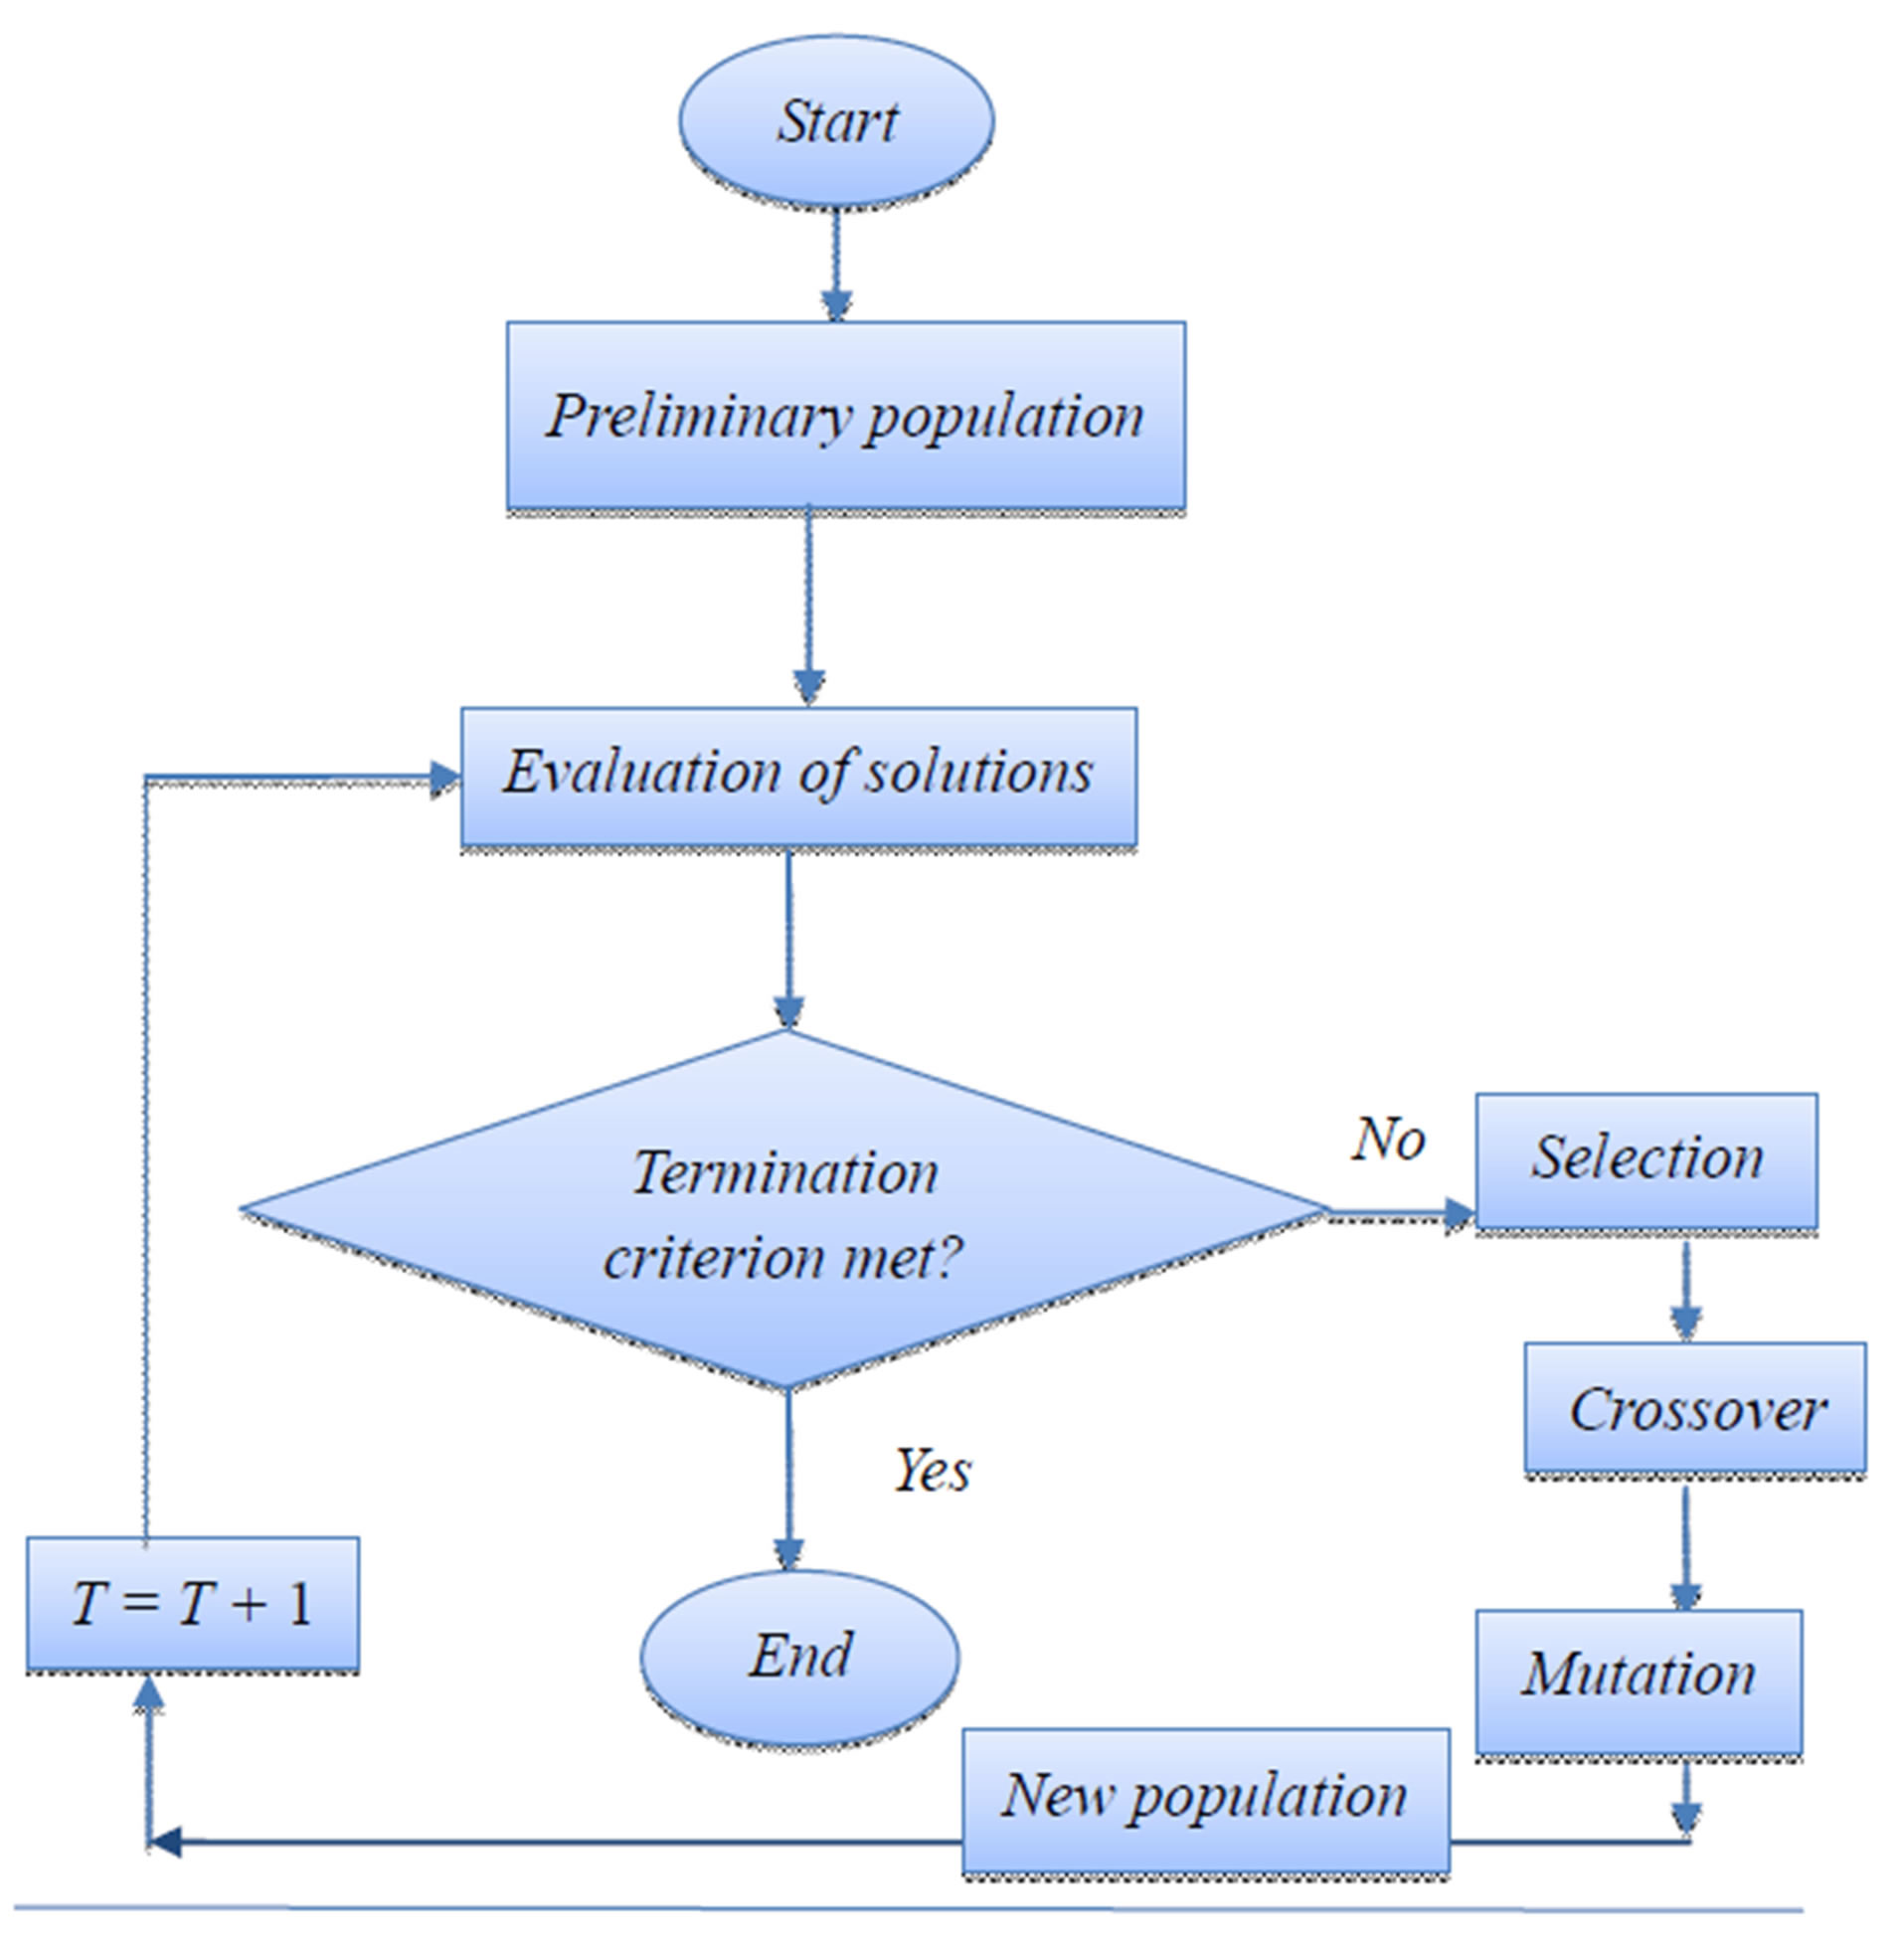
\includegraphics[width=0.6\linewidth]{figs/ga.jpg}
\\
\href{http://file.scirp.org/Html/1-8302163_41175.htm}{(Source)}
\end{center}

Once the algorithm is implemented, perform the following tasks:

\begin{enumerate}
	\item Show the best fitness found in each generation. Execute the algorithm. How does the best fitness evolve?
	\item Compare the execution time with $n=10$, $n=20$ and $n=100$. (Hint: Use the Unix command \texttt{time}).
\end{enumerate}

\end{document}

}{}

\section{EAs components}
\subsection{Components of an EA}
\begin{frame}{EAs components}{Components of an EA}
	Common components in any EA
	\begin{itemize}
		\item Representation
		\item Evaluation
		\item Selection
		\item Genetic operators
	\end{itemize}
\end{frame}

\subsection{Representation}
\begin{frame}{EAs components}{Representation (I)} 
	Main difference among EAs is the representation
	\begin{itemize}
		\item Strings: \alert{Genetic Algorithms (GA)}
		\item Real vectors: \alert{Evolution Strategies (ES)}
		\item State machine: \alert{Evolutive Programming (EP)}
		\item Trees: \alert{Genetic Programming (GP)}
	\end{itemize}
	These differences are, mostly, irrelevant
	\begin{itemize}
		\item Use the most natural representation
		\item Use the most natural genetic operators according to the representation
	\end{itemize}
\end{frame}

\begin{frame}{EAs components}{Representation (II)} 
	Example: 8 queens with a Genetic Algorithm
	\bigskip
    \begin{columns}
 	   \column{.50\textwidth}
	   \textbf{Phenotype}: Board position\\
	   \textbf{Genotype}: Integer vector
 	   \column{.50\textwidth}
		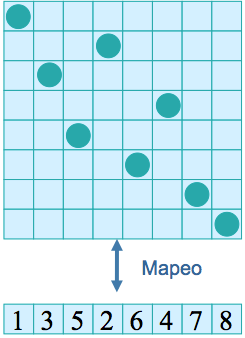
\includegraphics[width=0.7\linewidth]{figs/8queen.png}
	\end{columns}
\end{frame}

\begin{frame}{EAs components}{Representation (III)} 
	Example: Regression in Genetic Programming
	\bigskip
    \begin{columns}
 	   \column{.50\textwidth}
	   \textbf{Phenotype}: Tree\\
	   \textbf{Genotype}: Formula
 	   \column{.50\textwidth}
		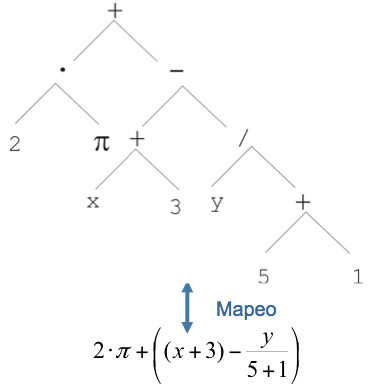
\includegraphics[width=\linewidth]{figs/gp.png}
	\end{columns}
\end{frame}

\subsection{Evaluation}

\begin{frame}{EAs components}{Evaluation (I)} 
	Individuals quality is assessed by a \alert{fitness function}
	\begin{itemize}
		\item Individual = Potential solution
	\end{itemize}
	The fitness assigns a numerical value to a phenotype
	\begin{itemize}
		\item Caution, phenotype, not genotype
		\item Multiobjective algorithms use several fitnesses
	\end{itemize}
	Evaluation uses to be a bottleneck
	\begin{itemize}
		\item Many times it involves simulating a system
	\end{itemize}
	Minimize number of evaluations
\end{frame}

\begin{frame}{EAs components}{Evaluation (II)} 
	Example: 8 queens
	\begin{itemize}
		\item The fitness may be the number of threaded pieces
		\item Objective: Minimize fitness (minimation problem)
	\end{itemize}
	Example: Regression
	\begin{itemize}
		\item The fitness may be the quadratic average error
		\item Objective: Minimize fitness (minimation problem)
	\end{itemize}
\end{frame}

\subsection{Selection}

\begin{frame}{EAs components}{Selection (I)} 
	Selection operator ``selects'' individuals for reproduction
	\begin{itemize}
		\item Imitates natural selection
		\item Higher reproduction probability for high fitness individuals
		\begin{itemize}
			\item Randomness helps avoiding local minima
		\end{itemize}
		\item Selection is done in phenotipic space!
		\begin{itemize}
			\item Selection does not take into account how representation is
		\end{itemize}
	\end{itemize}
	Introduces \alert{selective pressure}
\end{frame}

\begin{frame}{EAs components}{Selection (II)} 
	High selective pressure reduces \alert{genetic diversity}
	\begin{itemize}
		\item Faster evolution, higher probability of local maxima
		\item Eliminates low fitness individuals
		\begin{itemize}
			\item Potentially valuable genetic material can be lost
		\end{itemize}
		\item Selection operators: Tournment size $n$, roulette-wheel, rank-based, ...
	\end{itemize}
	
    \begin{columns}
    \column{0.5\textwidth}
	\begin{block}{Tournment size $n$}
	\begin{enumerate}
		\item Take randomly $n$ individuals
		\item Compute their fitness
		\item Select the highest fitness
	\end{enumerate}
	Variable selective pressure depending on $n$
    \end{block}
    \end{columns}
\end{frame}

\begin{frame}{EAs components}{Selection (III)} 
	Replacement strategy
	\begin{itemize}
		\item Select which individual replace
	\end{itemize}
	
	Two basic strategies
	\begin{itemize}
		\item Generational algorithms: Replace all the offspring
		\begin{itemize}
			\item Iterations are named \alert{generations}
			\item Time is usually measured in generations
		\end{itemize}
		\item Steady-stade: Replace part of the offscript
		\begin{itemize}
			\item Criteria: Age, fitness, selection, etc
			\item Lower memory consumption
		\end{itemize}
	\end{itemize}
	Hybrid strategy: \alert{Elitism}
		\begin{itemize}
			\item Replace the population, except the $n$ fittest individuals
			\item $n$ fittest individuals guaranteed to survive
		\end{itemize}
\end{frame}

\begin{frame}{EAs components}{Genetic operators (I)} 
	Genetic operators build new individuals
	\begin{itemize}
		\item Two basic operators: \alert{mutation} and \alert{crossover}
	\end{itemize}
	
	Open discussion (=research) about the role of mutation and crossover
	\begin{itemize}
		\item Mutation enhances exploration
		\item Crossover enhances explotation
	\end{itemize}

	Both are used
	\begin{itemize}
		\item Historial constrains
	\end{itemize}
\end{frame}

\subsection{Genetic operators}

\begin{frame}{EAs components}{Genetic operators (II)} 
	Mutation operator
	\begin{itemize}
		\item It takes a genotype and returns another one
		\begin{itemize}
			\item It has a stochastic behavior
			\item Used to maintain genetic diversity
		\end{itemize}
		\item Guarantees search space connectivity 
		\item Mutation plays a disruptive role
		\begin{itemize}
			\item Moves population to new regions
		\end{itemize}
	\end{itemize}
	
	Example: 8 queens permutation operator
	\begin{center}
		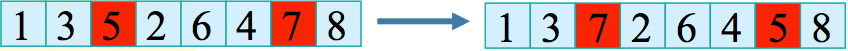
\includegraphics[width=0.7\linewidth]{figs/permutacion.png}
	\end{center}
\end{frame}

\begin{frame}{EAs components}{Genetic operators (III)} 
	Crossover operator
	\begin{itemize}
		\item Fuse information from the parents (sexual reproduction)
		\begin{itemize}
			\item Randomness has a place 
		\end{itemize}
		\item Offspring uses to be worse than its parents
		\begin{itemize}
			\item With luck, good components of the parents are joined ...
			\item ... and this is something that happens
		\end{itemize}
		\item Crossover has a constructive role
		\begin{itemize}
			\item Join preexistent components
			\item Does not generate new genetic material
			\item Encourages explotation
		\end{itemize}
	\end{itemize}
\end{frame}

\begin{frame}{EAs components}{Genetic operators (IV)} 
	Example: 8 queens with one-point crossover
	\begin{center}
		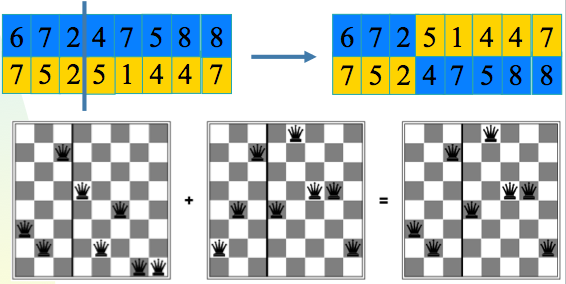
\includegraphics[width=0.7\linewidth]{figs/one-point.png}
	\end{center}
\end{frame}

\section{Working with an Evolutionary Algorithm}
\subsection{Search phases}
\begin{frame}{Working with an Evolutionary Algorithm}{Search phases}
    \begin{columns}
 	   \column{.70\textwidth}
	   \textbf{Initial phase}: Random distribution, high genetic diversity\\
	   \textbf{Advanced phase}: Begins to converge\\
	   \textbf{Convergence}: Around one or few points, low genetic diversity\\
	   \bigskip
	   Premature convergence if population not located in global maxima
 	   \column{.30\textwidth}
		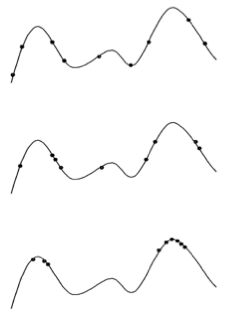
\includegraphics[width=\linewidth]{figs/fases.png}\\
		\centering\href{https://upload.wikimedia.org/wikipedia/commons/f/fe/Visualization\_of\_a\_population\_evolving\_in\_a\_static\_fitness\_landscape.gif}{(Animation)}
	\end{columns}
\end{frame}

\subsection{Fitness dynamics}
\begin{frame}{Working with an Evolutionary Algorithm}{Fitness dynamics}
    \begin{columns}
 	   \column{.50\textwidth}
		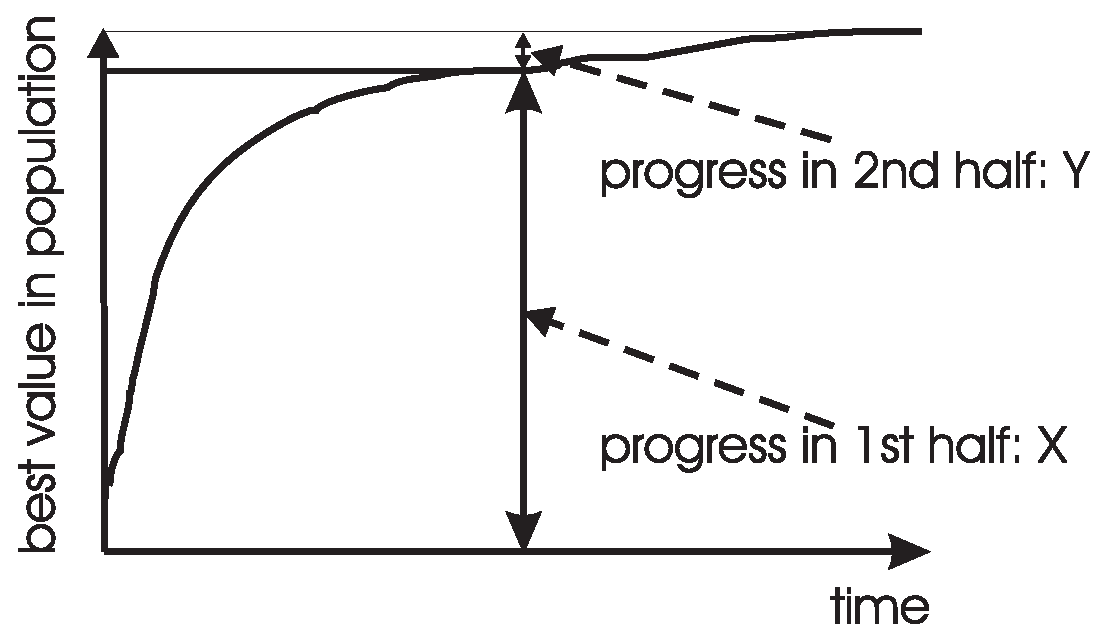
\includegraphics[width=\linewidth]{figs/fitness.eps}
 	   \column{.50\textwidth}
		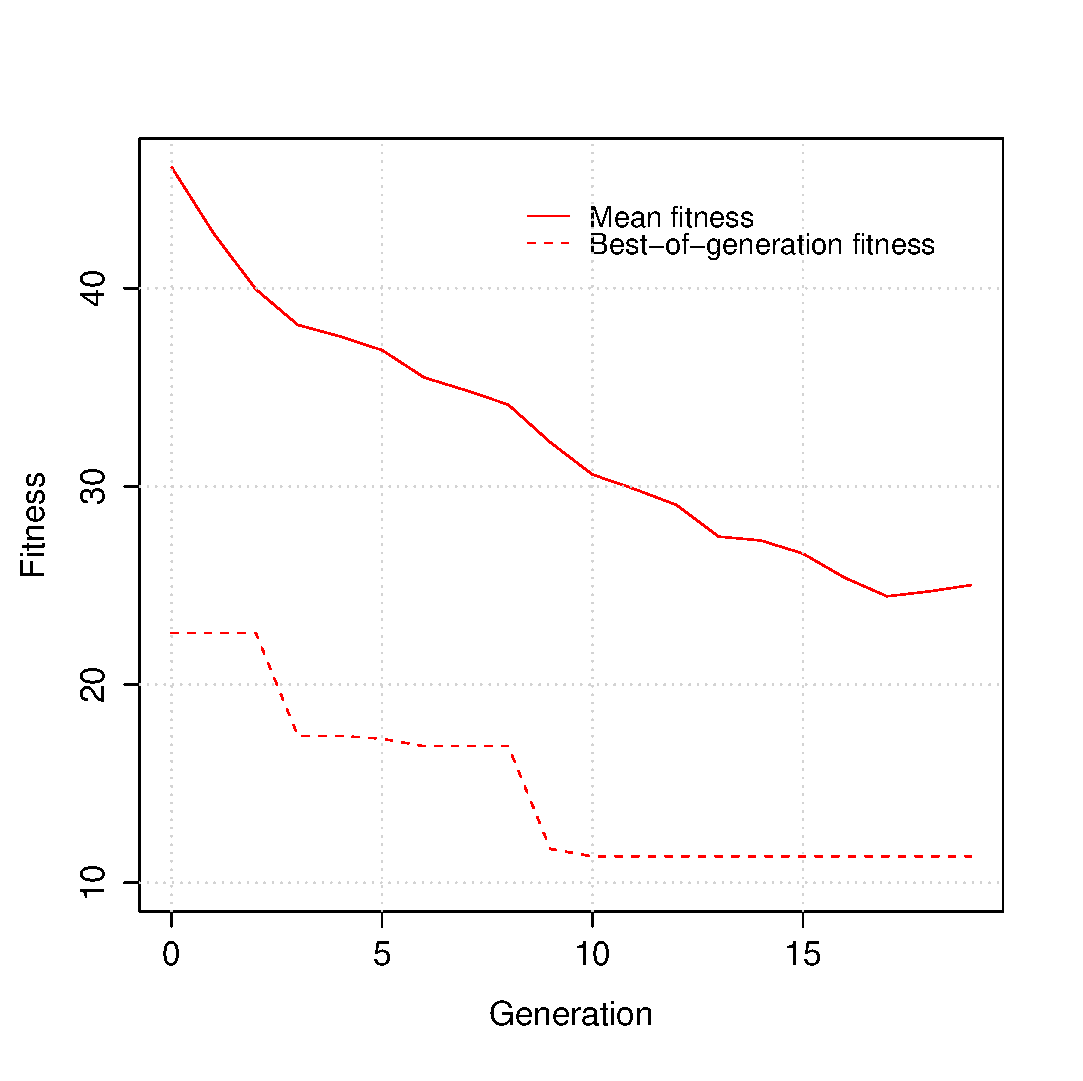
\includegraphics[width=\linewidth]{figs/fitness-k2.eps}
	\end{columns}
	Few long runs or many short runs?
\end{frame}

\subsection{When  EAs are useful}
\begin{frame}{Working with an Evolutionary Algorithm}{When EAs are useful}
    \begin{columns}
 	   \column{.70\textwidth}
		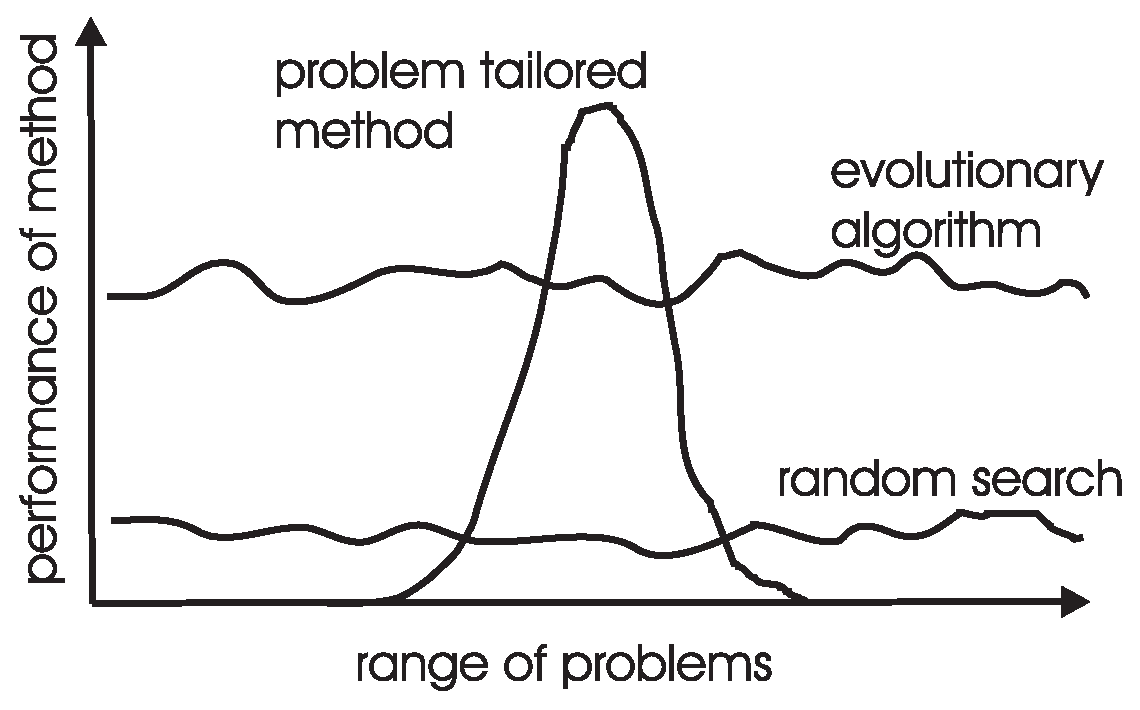
\includegraphics[width=\linewidth]{figs/problems.eps}
	\end{columns}
\end{frame}

\subsection{Advanced EAs}
\begin{frame}{Working with an Evolutionary Algorithm}{Advanced EAs}
	\begin{itemize}
	\item Multiobjective Evolutionary Algorithms (MOEAs)
	\item Optimization with constrains
	\item Coevolution
	\item Dinamic optimization
	\item Islands models
	\item Memetic algorithms
	\item Hyperheuristics
	\end{itemize}
\end{frame}

\subsection{EAs examples}
\begin{frame}{Working with an Evolutionary Algorithm}{Examples}
	\begin{itemize}
		\item \href{http://rednuht.org/genetic\_cars\_2/} {(Car design)}
		\item \href{http://rednuht.org/genetic\_walkers/} {(Genetic Algorithm Walkers)}
		\item \href{http://www.blprnt.com/smartrockets/}{(Smart rockets)}
		\item \href{https://www.youtube.com/watch?v=xcIBoPuNIiw}{(Learn to walk)}
		\item \href{https://www.youtube.com/watch?v=pgaEE27nsQw}{(Flexible Muscle-Based Locomotion for Bipedal Creatures)}
		\item \href{https://www.youtube.com/watch?v=qv6UVOQ0F44}{(MarI/O - Machine Learning for Video Games)}
		\item \href{https://www.youtube.com/watch?v=u2t77mQmJiY}{(A genetic algorithm learns how to fight!)}
		\item \href{https://www.youtube.com/watch?v=HgWQ-gPIvt4}{(Evolved Electrophysiological Soft Robots)}
	\end{itemize}
\end{frame}


\end{document}
